\documentclass[11pt]{book}
\usepackage{graphicx}
\usepackage{wrapfig}
\usepackage{amsmath}
\usepackage{longtable}
\usepackage[table]{xcolor}
\usepackage{amssymb}
\usepackage[rightcaption]{sidecap}
\usepackage{ upgreek }
\begin{document}
\bibliographystyle{plain}
\begin{titlepage}
\centering
	{\scshape\LARGE Uniwersytet Gdanski\par}
	\vspace{1cm}
	{\scshape\Large Projekt LATEX\par}
	\vspace{1.5cm}
	{\huge\bfseries Przykladowa ksiazka\par}
	\vspace{2cm}
	{\Large\itshape Michal Olkiewicz\par}
	\vfill
	{\large \today\par}
\end{titlepage}
\chapter{First Crusade}
\begin{quote}
... and the people respond as with one voice:
\newline
Dues vult!
\newline
God wills it!
\end{quote}
-Pope Urban II
\newpage
\section{General Info}
List of events:
\begin{enumerate}
   \item Council of Clermont
   \begin{itemize}
     \item Recruitment
   \end{itemize}
   \item People's Crusade
   \begin{itemize}
   	\item Attacks on Jews in the Rhineland
   \end{itemize}
   \item Princes' Crusade \cite{CrusadeBook1}
   \begin{itemize}
   	\item Siege of Nicaea
   	\item Battle of Dorylaeum
   	\item Siege of Antioch
   	\item Continued march to Jerusalem
   	\item Siege of Jerusalem
   	\item Establishment of the Kingdom of Jerusalem
   	\item  Battle of Ascalon
   \end{itemize}
   \item Crusade of 1101
\end{enumerate}
\newpage
 \begin{longtable}[c]{| c | c |}
\caption{Statistics for the First Crusade} \label{tab:statsFirstCrusade} \\
 \hline
 \multicolumn{2}{| c |}{Beligerents}\\
 \hline
 Crusaders& Islam Forces\\
 \hline
 \endfirsthead
  \hline
 \multicolumn{2}{|c|}{Commanders and leaders} \\
 \hline
 Crusaders& Islam Forces\\
 \hline
 \endhead
 
 \hline
 \endfoot
 
 \hline
 \endlastfoot
   
 Kingdom of France   & Seljuk Sultanate    \\
 Blois&   Danishmends\\
 Toulouse &Fatimid Caliphate\\
 Boulogne&Abbasid Caliphate\\
 Flanders&\\
 Kingdom of England&  \\
 Normandy&\\
 Le Puy-en-Velay&\\
 Vermandois&\\
 Brittany&\\
 Republic of Genoa&\\
 Armenian Cilicia&\\
 County of Sicily&\\
 Taranto&\\
 Roman (Byzantine) Empire&\\
  \hline
 \multicolumn{2}{|c|}{Commanders and leaders} \\
 \hline
  Crusaders& Islam Forces\\
 \hline
 
German Contingent: & \\
Godfrey of Bouillon & Kilij Arslan I\\
Baldwin of Boulogne & Yaghi-Siyan \\
Southern French Contingent: & \\
Raymond IV of Toulouse & Kerbogha \\
Adhemar of Le Puy & Duqaq \\
Hugh I of Vermandois & Fakhr al-Mulk Radwan \\
Northern French Contingent:  & \\
Stephen II of Blois & Ghazi ibn Danishmend \\
Robert II of Flanders & Iftikhar ad-Daula \\
Robert II of Normandy & Al-Afdal Shahanshah \\
Norman-Italian Contingent: & \\
Bohemond of Taranto &	\\
Tancred of Hauteville & \\
Eastern Leaders: & \\
Alexios I Komnenos & \\
Tatikios & \\
Manuel Boutoumites & \\
Constantine of Armenia & \\
Others: & \\
Guglielmo Embriaco & \\ 
  \hline
 \multicolumn{2}{|c|}{Strength} \\
 \hline
  Crusaders& Islam Forces\\
 \hline
Crusaders:~ 35,000 men & Unknown \\
30,000 infantry & \\
5,000 cavalry knights & \\
Byzantines:~ 2,000 men & \\
  \hline
 \multicolumn{2}{|c|}{Casualties and losses} \\
 \hline
   Crusaders& Islam Forces\\
 \hline
 Moderate to High (estimates vary) & High \\
\end{longtable}
\cite{CrusadeBook4}
\begin{SCfigure}[0.5][h]
\caption{A drawing of a crusader}
\centering
\label{fig:pictureofcrusader}
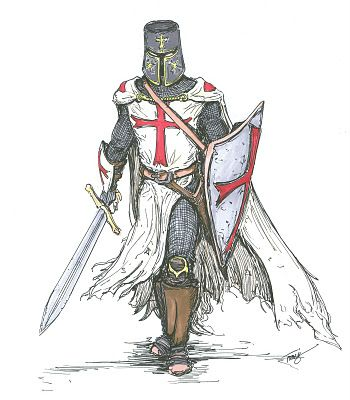
\includegraphics[width=0.5\textwidth]{one}
\end{SCfigure}
\chapter{Second Crusade}
\begin{quote}
Si Vis Pachem Para Bellum!
\end{quote}
-Unknown
\newpage
\section{General Info}
Important facts:
\begin{enumerate}
\item The fall of Edessa
\item  Saint Bernard of Clairvaux
\item Wendish Crusade
\item Reconquista and the fall of Lisbon
\item Crusade in the East \cite{CrusadeBook2}
\begin{itemize}
	\item Routes:
	\begin{itemize}
	\item German route
	\item French route
	\end{itemize}
	\item Journey to Jerusalem
	 \item  Council of Acre
	 \item Siege of Damascus
\end{itemize}
\end{enumerate}
\newpage
\begin{table}
\begin{center}
\caption{Statistics for the Second Crusade}
\label{tab:statsSecondCrusade}


\begin{tabular}{ |p{3cm}|p{3cm}|p{3cm}|p{3cm}|  }
 \hline
 \multicolumn{4}{|c|}{Country List} \\
 \hline
 \multicolumn{2}{|c|}{Belligerents} & \multicolumn{2}{c|}{Commanders and leaders}\\
 \hline
 Crusaders & Islam Forces & Crusaders & Islam Forces \\
 \hline
 Kingdom of Jerusalem&Seljuq Sultanate&Melisende of Jerusalem&Mesud I\\
 County of Tripoli&Emirate of Zengids& Baldwin III of Jerusalem& Imad ad-Din Zengi\\
 Principality of Antioch&Abbasid Caliphate&Raymond II of Tripoli&Nur ad-Din\\
 Knights Templar &Fatimid Caliphate&Raymond of Poitiers&Saif ad-Din Ghazi I\\
 Knights Hospitaller&Nizari Ismailis of Syria &Louis VII of France&Al-Muqtafi\\
 Canons Regular of the Holy Sepulchre&Almoravids&Thoros II of Armenia&Al-Hafiz\\
  Knights of Saint Lazarus&Taifa of Valencia&Raynald of Châtillon&Tashfin ibn Ali\\
   Kingdom of France&Taifa of Murcia&Theodwin&Ibrahim ibn Tashfin \\
    Holy Roman Empire&Obotrite Confederacy&Afonso I of Portugal&Ishaq ibn Ali\\
    Byzantine Empire&Liutizian Confederacy&Alfonso VII of León and Castile&Abd al-Mu'min\\
    Kingdom of England&Duchy of Pomerania&Ramon Berenguer IV&Niklot\\
    Kingdom of Sicily& &Conrad III of Germany&Pribislav of Wagria\\
    Papal States&  &Ottokar III of Styria&Ratibor I of Pomerania\\
    Kingdom of Poland&  &Stephen, King of England&\\
 \hline
 \multicolumn{4}{|c|}{Strength} \\
 \hline
 Germans: 20,000 men & French: 15,000 men & \multicolumn{2}{c|}{}\\
 \hline
\end{tabular}


\end{center}
\end{table}
\begin{figure}
\caption{A drawing of Raymond of Poitiers welcoming Louis VII  in Antioch}
\centering
\label{fig:pictureofsecondcrusade}
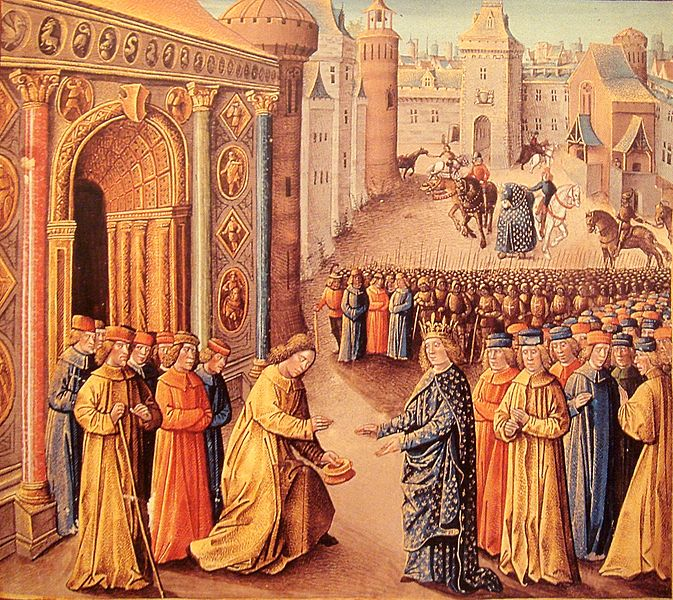
\includegraphics[width=\textwidth]{two}
\end{figure}
\chapter{Third Crusade}
\begin{quote}
Justtitia suum cuique distribuit
\end{quote}
-Unknown
\newpage
\section{General Info}
List of events:
\begin{enumerate}
\item Barbarossa's crusade \cite{CrusadeBook3}
\item Departure
\begin{enumerate}
\item King Richard Departure
\item King Philip's Departure
\end{enumerate}
\item Siege of Acre
\item Battle of Arsuf
\item Advances on Jerusalem, regicide, and negotiations
\end{enumerate}
\newpage
\setlength{\arrayrulewidth}{0.5mm}
\setlength{\tabcolsep}{24pt}
\renewcommand{\arraystretch}{2.5}
\begin{wraptable}{l}{8cm}
\centering
\caption{Statistics for the Third Crusade}
\label{tab:statsThirdCrusade}
{\rowcolors{1}{red!100!gray!30}{red!50!gray!90}
\begin{tabular}{ |p{1.5cm}|p{2cm}|p{1.5cm}|p{1cm}|p{1.5cm}|  }
\hline
\multicolumn{5}{|c|}{Third Crusade} \\
\hline
\multicolumn{2}{|c|}{Belligerents} & \multicolumn{2}{c|}{Commanders and leaders} & Strength\\
\hline
Crusaders & Islam Forces & Crusaders &Islam Forces&Crusaders \\
\hline
Kingdom of England&Ayyubid Sultanate &King Richard the Lionheart&Sultan Saladin&English: 8,000 men \\
Kingdom of France&Sultanate of Egypt&King Philip Augustus&Al-Muzaffar Umar&French: 2,000 men \\
Duchy of Burgundy&Emirate of Damascus&Duke Hugh III of Burgundy&Al-Adil I&Germans: 15,000-100,000 men \\
County of Blois&Emirate of Hama&Count Theobald V of Blois&Al-Afdal&Hungarians: 2,000 men\\
Holy Roman Empire&Emirate of Mesopotamia&Count Henry II of Champagne&Robert of St. Albans&\\
Duchy of Swabia&Sultanate of Rum&Guy of Lusignan& &\\
Duchy of Austria&Nizari Ismaili state& & &\\
\hline
\end{tabular}
}
\end{wraptable}
\newpage
\begin{wrapfigure}{l}{8cm}
\begin{center}
\caption{A drawing of The Siege of Acre}
\centering
\label{fig:pictureofacre}
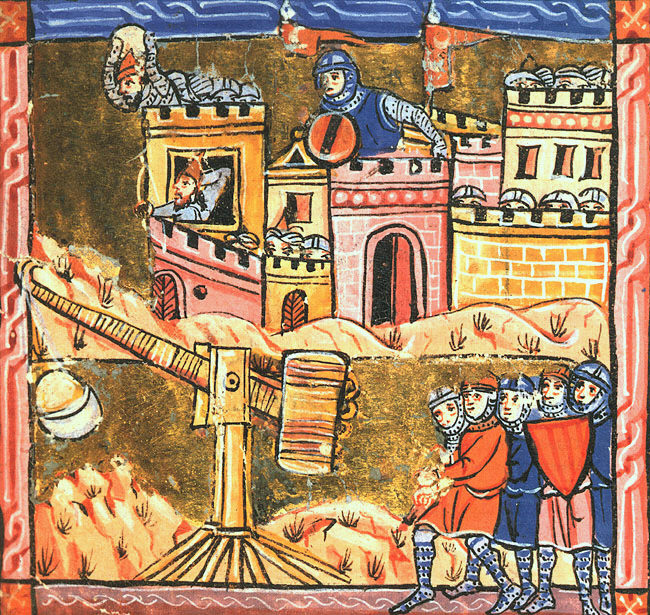
\includegraphics[scale=1.5]{three}
\end{center}
\end{wrapfigure}
\newpage
\chapter{Additional Information}
Lorem ipsum dolor sit amet, consectetur adipiscing elit, sed do eiusmod tempor incididunt ut labore et dolore magna aliqua. Ut enim ad minim veniam, quis nostrud exercitation ullamco laboris nisi ut aliquip ex ea commodo consequat. Duis aute irure dolor in reprehenderit in voluptate velit esse cillum dolore eu fugiat nulla pariatur. Excepteur sint occaecat cupidatat non proident, sunt in culpa qui officia deserunt mollit anim id est laborum. \cite{article1}
\newpage
\section{Trebuchet}
Mathematics behind Trebuchet:\\
The coordinates of the counterweight M are given as:
$$x_M = -L_1 \sin \theta - L_4 \sin (- \theta - \beta) $$ 
$$x_M = -L_1 \sin \theta + L_4 \sin (\theta + \beta) $$
$$y_M = L_1 \cos \theta - L_4 \cos (- \theta - \beta) $$
$$y_M = L_1 \sin \theta - L_4 \sin ( \theta + \beta) $$
The acceleration of the counterweight M is: 	
$$ a_Mx = \frac{d^2x_M}{dt^2} $$
$$ a_My = \frac{d^2y_M}{dt^2} $$
By Newton's Second Law,
$$ \Upsigma\bar{F}_x = M(\bar{a}_Mx) $$
$$ \Upsigma\bar{F}_y = M(\bar{a}_My) $$
where M is the mass of the counterweight. \\

Therefore,
$$ T_2 \sin(-\theta - \beta) =Ma_Mx $$ 
$$ - T_2 \sin(\theta + \beta) =Ma_Mx $$ 
$$ T_2 \cos(-\theta - \beta) - M_g =Ma_My $$ 
$$ T_2 \cos( \theta + \beta) - M_g =Ma_My $$ 
\cite{online1}
\newpage
\begin{figure}
\begin{center}
\caption{A drawing of a Trebuchet}
\centering
\label{fig:pictureoftrebuchet}
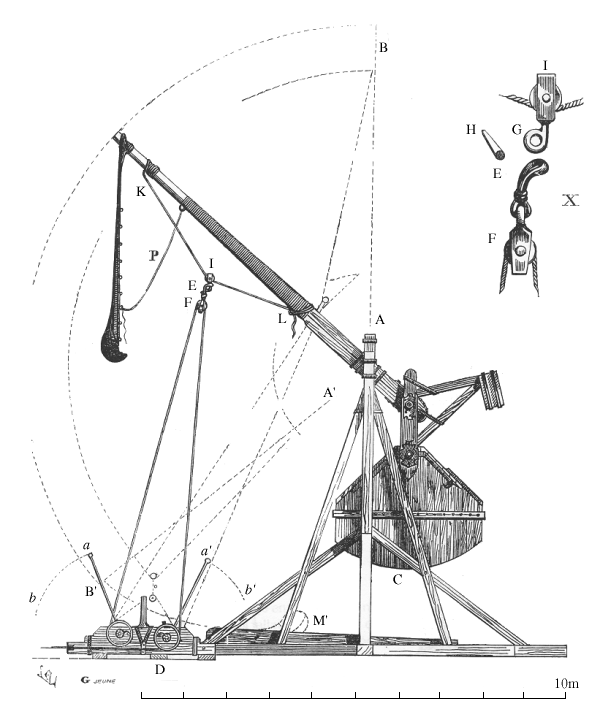
\includegraphics[scale=0.5, angle=45]{four}
\end{center}
\end{figure}
\section{Mathematics}
\subsection{The Callan-Symanzik equation}
\begin{equation}
[M \frac{\partial}{\partial M}+ \beta(g)\frac{\partial}{\partial g}+n\gamma]G^n(x_1,x_2, ... ,x_n;M,g)=0
\end{equation}
\subsection{The minimal surface equation}
\begin{equation}
A(u) = \int\limits_\Omega (1+ |\bigtriangledown u|^2)^\frac{1}{2} dx_1 ... dx_n
\end{equation}
\subsection{Standard model}
\begin{equation}
\begin{split}
\mathcal{L}_SM =
&\frac{1}{4}W_{\mu\nu} \cdot W^{\mu\nu} - q\frac{1}{4}B_{\mu\nu} B^{\mu\nu}-\frac{1}{4}G^a_{\mu\nu} G^{\mu\nu}_a \\
 & + \bar{L}\upgamma^\mu(i\partial \mu - \frac{1}{2}g\tau \cdot W_\mu - \frac{1}{2}\mu)L \\
 & + \bar{R}\upgamma^\mu(i\partial \mu - \frac{1}{2}g'YB_\mu)R \\
 & + \frac{1}{2}|(i\partial_\mu - \frac{1}{2}g\tau \cdot W_\mu - \frac{1}{2}g'YB_\mu )\phi|^2 V(\phi)\\
 & + g''(\bar{q}\tau^\mu T_aq) G_\mu^a + (G_1\bar{L}\phi R + G_2\bar{L}\phi_cR + h.c.)\\
\end{split}
\end{equation}
\cite{MathBook}
\tableofcontents
\listoftables
\listoffigures
\bibliography{bibliografia}
\end{document}